\chapter{Die Skelettierung}
\Autor{Sandra Schröder}\\\\
TODO: Genaue Theorie zur Skelettierung. Eigenschaften. Abhängig von Verfahren blaaaaaaaaaaa
Dieses Kapitel beschreibt bekannte Konzepte und Verfahren zur Skelettierung im Bereich der Bildverarbeitung.\\
Zwei Verfahren sind im Rahmen der Projektarbeit besonders wichtig: Das \emph{Thinning} (deutsch: Verdünnung) und die \emph{Distanztransformation}. \\
Um die Übersicht über die weiteren grundlegenden Verfahren und Konzepte zu vervollständigen, werden diese in einem separaten 
Abschnitt kurz vorgestellt.
\section{Thinning}
\Autor{Johannes Böhler}\\
Das Thinning bezeichnet eine Kategorie von Methoden zur Skelettierung von 2D sowie 3D Objekten. In dieser Projektarbeit ist der Fokus ausschliesslich auf die 2D Skelettierung gerichtet, da die Kinect kein vollkommenes 3D Modell eines Objektes liefert. Sie erfasst das Objekt lediglich aus einem Blickwinkel, desshalb erhält man nur ein 2,5 dimensionales Modell. Es werden nur Tiefeninformationen bezüglich der Seite des Objektes, welche der Kinect zugewendet ist bereitgestellt. Die  Tiefeninformationen der Rückseite bleiben verborgen. Um ein vollständiges 3D Modell zu erhalten müssten mindestens 2 Kinects verwendet werden und die Informationen beider Geräte zusammengeführt und vereinheitlicht werden. 

Alle Thinning Algorithmen verbindet das iterative Abtragen des Musters oder der Oberfläche.
\newpage
\section{Distanztransformation}
\Autor{Sandra Schröder}\\\\
Die Distanztransformation eines Binärbildes enthält Informationen über den Abstand der Objektpixel zum Hintergrund. Der Abstand zum Hintergrund wird für jeden Objektpixel bestimmt und in einem
weiteren Bild (gleiche Dimension und Größe wie das Binärbild) als Grauwert an der Stelle des Objektpixels gespeichert. Das Ergebnis ist die sogenannte \emph{Distance Map} (Distanzkarte). \\
Zur Bestimmung des Abstands benötigt man Metriken. Eine gängige Metrik - die für den Algorithmus im Rahmen dieser Arbeit auch genutzt wurde - ist die euklidische Metrik $d_2$ \textbf{TODO Quelle} (Gleichung \ref{eq:d2}):
\begin{equation}
\label{eq:d2}
d_2(p,q) = \sqrt{(p_x - q_x)^2 + (p_y - q_y)^2}  
\end{equation}
Die Definition einer Nachbarschaft spielt
ebenfalls eine Rolle. Wählt man eine
4er-Nachbarschaft, wird der Abstand vom Objektpixel zur linken und zur rechten Seite, sowie nach oben und nach unten berechnet. Man erhält dementsprechend
vier Abstände. In der Distance Map wird der minimale Abstand von den vier Werten
gespeichert. Bei einer 8er-Nachbarschaft
kommen die diagonalen Richtungen dazu.\\
Die Distance Map wird zur Extraktion des Skeletts benutzt. Die
Pixel die im Objekt beziehungsweise in Objektregionen mittig liegen, besitzen den größten Abstand zum Hintergrund relativ zu den unmittelbaren Pixeln. Die Pixel mit dem größten Abstand sind dementsprechend die hellsten Pixel in der Distancemap. Betrachtet man diesen Teil der Distance Map beschreibt dieser ein potentielles Skelett.
\label{sec:distanztransformation}
\begin{figure}[h]
	\centering
	\begin{minipage}{4cm}
		\centering
		
\includegraphics[width=1.0\linewidth]{./fig/person.jpg}
		\label{fig:beispiel_person}
	\end{minipage}
	\hspace{3cm}
	\begin{minipage}{4cm}
		\centering
		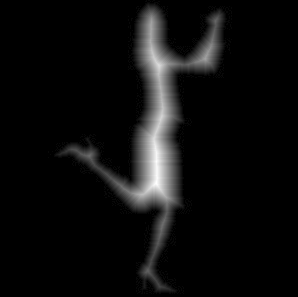
\includegraphics[width=1.0\linewidth]{./fig/distance_map_beispiel}	
	\end{minipage}
	\caption{Beispiel einer Distance Map. Links: Originalbild. Dieses wurde zuerst invertiert, damit das Objekt (Person) weiß markiert ist. Rechts: Resultat der Distanztransformation. Aufällig ist das Maximum in der Mitte.}
	\label{fig:distance_map_beispiel}
\end{figure}
\subsection{Extraktion des Skeletts}
Es stellt sich die Frage, wie das Skelett extrahiert werden kann. Betrachtet man die Struktur einer
Distance Map, wie zum Beispiel in Abbildung \ref{fig:distance_map_beispiel}, erkennt man, dass die Pixel,
die in der Mitte des Objektes liegen, den größten Abstand zum Hintergrund haben. Die Distance Map bildet ein Grauwertgebirge. Diese Information wird ausgenutzt, um die Skelettlinie, das heißt die höchste Stelle
im Grauwertgebirge, zu extrahieren. \\
Die Idee ist, den Gradienten der Distance Map zu bestimmen. Der Gradient (Gleichung \ref{eq:gradient}) ist ein Differentialoperator und liefert, angewandt auf ein Skalarfeld, die Richtung des stärksten Anstiegs, sowie die Amplitude des Anstiegs (Gradientenbetrag):
\begin{equation}
\label{eq:gradient}
%      \[
   grad(f(x,y)) = \nabla f(x,y) = \begin{bmatrix}
         \frac{df}{dx}        \\[0.3em]
         \frac{df}{dy} \\[0.3em]
      \end{bmatrix}
%  \]
\end{equation}
Ein Graubild kann als skalare Funktion $f(x,y)$ beschrieben werden mit $x,y \in \mathbb{N}$ und
$0 \leq f(x,y) \leq 255$. Somit lässt sich der Gradient auch auf Graubilder übertragen.
Entsprechend der Definition des Gradienten, ist an der höchsten Stelle des Grauwertgebirges der Gradientenbetrag gleich null.\\
Kodiert man den Gradientenbetrag ebenfalls als ein Grauwertbild, wird der Gebirgskamm eine schwarze Linie
sein und das potentielle Skelett markieren. Segmentierung des Gradientenbetragbildes. Skelett schwarz, anderer Bereich ist weiß (außer Hintergrund). Dann Differenz bilden mit Distanz Map. Ergibt Skelett. 
\section{Weitere Verfahren}
\Autor{Christopher Kroll}